\subsection{Theory Exercises}

\subsubsection*{Bishop 11.3}

To transform a random variable \( z \sim \text{Uniform}(0, 1) \) into a random variable \( y \) with the Cauchy distribution 
\[
p(y) = \frac{1}{\pi} \frac{1}{1 + y^2},
\]
We Firstly determine the CDF of the Cauchy distribution
\[
F_Y(y) = \int_{-\infty}^y \frac{1}{\pi} \frac{1}{1 + t^2} \, dt = \frac{1}{\pi} \arctan(y) + \frac{1}{2}.
\]
To map \( z \sim \text{Uniform}(0, 1) \) to \( y \sim p(y) \), we set:
\[
F_Y(y) = z.
\]
And solve for y
\[
\frac{1}{\pi} \arctan(y) + \frac{1}{2} = z.
\]
\[
\arctan(y) = \pi z - \frac{\pi}{2}.
\]
Taking the tangent of both sides:
\[
y = \tan\left(\pi z - \frac{\pi}{2}\right).
\]
We can conclude that the transformation is given by:
\[
y = \tan\left(\pi z - \frac{\pi}{2}\right) \quad \text{or equivalently} \quad y = -\cot(\pi z).
\]


\subsection{Programming Exercise}

\subsection{Pyro}

The code is shown in~\cref{sec:week3:code:pyro}.
The plot of the GMM samples is shown in~\cref{fig:week3:pyro:gmm-samples}.
The plots of the densities $p(x_2 | x_1 = 2)$ and $p(x_2 | x_1 = 3)$
are shown in~\cref{fig:week3:pyro:cond-pdf}.

\begin{figure}[htbp]
  \centering
  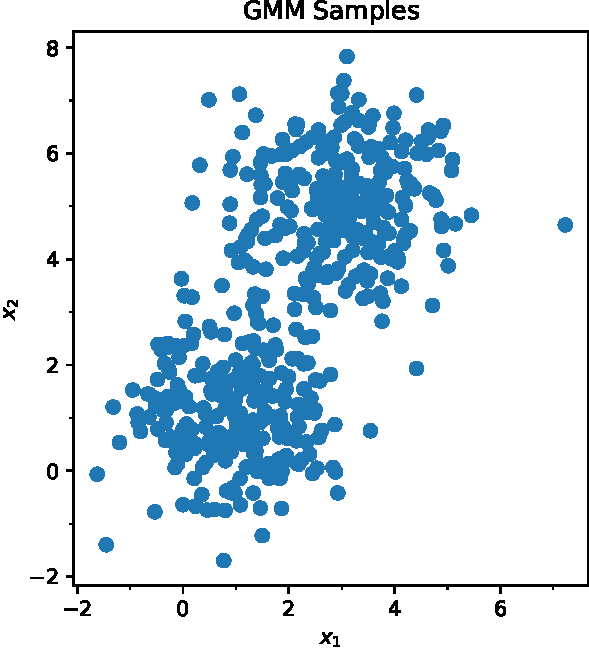
\includegraphics[width=0.5\textwidth]{./figures/gmm_samples.pdf}
  \caption{Scatter plot of 500 samples of the GMM.}
  \label{fig:week3:pyro:gmm-samples}
\end{figure}

\begin{figure}[htbp]
  \centering
  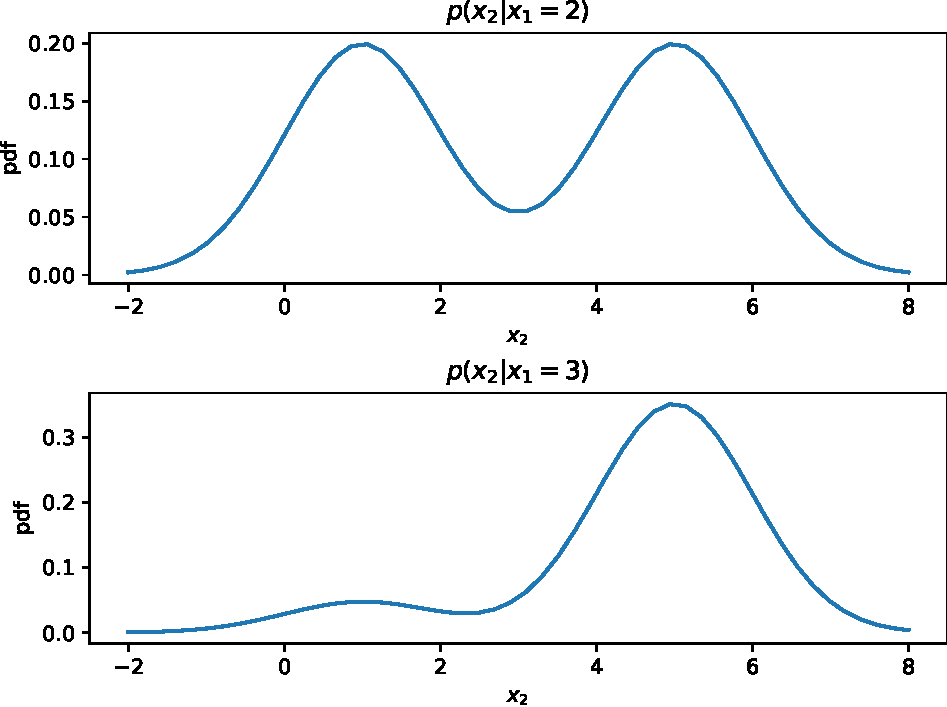
\includegraphics[width=0.7\textwidth]{./figures/cond_pdf.pdf}
  \caption{
    PDF of conditionals on $x_1$ of the GMM.
  }
  \label{fig:week3:pyro:cond-pdf}
\end{figure}
